\section{法兰盘三视图}

{\bfseries 知识目标}
\begin{itemize}
\item 掌握回转体三视图规律
\end{itemize}

{\bfseries 技能目标}
\begin{itemize}
\item 能够应用三视图对应关系,运用AutoCAD绘制回转体的三视图
\end{itemize}

图\ref{fig:falanpanlititu}所示为工业中应用泛用于管道连接的法兰盘零件的简化形式。本任务主要是让读者了解并掌握回转体三视图表述方式,实现应用AutoCAD进行回转体类零件的三视图绘制的技能目标。
\begin{figure}[htbp]
\centering
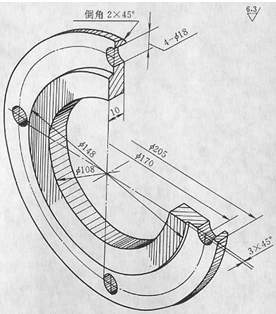
\includegraphics[scale=1]{fananlititu.png}
\caption{法兰盘}\label{fig:falanpanlititu}
\end{figure}


\endinput